% zweiseitiger druck -> bindung
\documentclass[a4paper,10pt,twoside,ngerman,bibliography=totoc]{scrreprt}
% einseitiger druck -> ebook
% \documentclass[a4paper,11pt,oneside,ngerman,bibliography=totoc]{scrreprt}

\usepackage{babel}                          % deutsche Trennmuster
% \usepackage{ae}                           % beseitigt Fehler beim pdf erzeugen

\usepackage[T1]{fontenc}                    % T1-kodierte Schriften, korrekte Trennmuster fuer Worte mit Umlauten
\usepackage[utf8]{inputenc}
\usepackage[default]{opensans}
\usepackage{courier}                        % Courier\ttdefault
\usepackage{microtype}
\usepackage{mathswap}

\usepackage{amsmath,amsthm,amsfonts,amssymb}
\usepackage{esint}                          %schöne integrale, benötigt amsmath

\usepackage{wrapfig}                        % text um bilder fliesen lassen
\usepackage{longtable}
\usepackage{booktabs}
\usepackage{color}                          % Schriftfarbe
\usepackage{lscape}
\usepackage{subfigure}
\usepackage[subfigure]{tocloft}
\usepackage{appendix}
\usepackage{caption}
\usepackage{graphicx}
\usepackage{setspace}
% \usepackage{subfig}
\usepackage{pdfpages}
\usepackage{verbatim}
\usepackage[tight,ugly]{units}
% \usepackage{lmodern}
\usepackage{hyperref}              %links an referenzen setzen

% \usepackage{amsmath}
% \usepackage{graphicx}
% \usepackage{array}
% \usepackage{MnSymbol}
% \usepackage{url}
% \usepackage{here}
% \usepackage{arydshln}


% packages für Programmablaufplan
\usepackage{tikz}
\usetikzlibrary{shapes,arrows}
\usepgflibrary{arrows}

% packages für Programmablaufplan
\usepackage{tikz}
\usetikzlibrary{shapes,arrows}
\usepgflibrary{arrows}

%plus(minus)
% \usepackage{relsize}
% \newcommand*\myPM{\ensuremath{\substack{+\\[-0.25em]-}\,}}
% \newcommand*\myPMbM{\ensuremath{\substack{+\\[-0.25em]\mathsmaller(-\mathsmaller)}\,}}
% \newcommand*\myPMbP{\ensuremath{\substack{\mathsmaller(+\mathsmaller)\\[-0.25em]-}\,}}

% defninierte Farben
\definecolor{fond}{RGB}{240,240,240}

\renewcommand{\vec}[1]{\boldsymbol{\mathrm{#1}}}
\renewcommand{\b}[1]{\mathbf{#1}}
\newcommand{\its}{\it\sffamily}
\renewcommand{\captionlabelfont}{\bfseries\sffamily}                                                          % Bildunterschriften fett, sf-Schriftart
\renewcommand{\captionfont}{\sffamily}                                                                          % Bildunterschriften sf-Schriftart
\captionsetup[table]{singlelinecheck = true, aboveskip=0pt, belowskip=7pt}  % Format Tabellenüberschriften
\newcommand{\tabformat}{\small\sffamily}                                                                        % Serifenlose und kleine Schrift in Tabelle
\renewcommand{\arraystretch}{1.4}                                                                                       % Groessere Abstaende zwischen Zeilen in Tabelle

% Seitenaufbau
\setstretch{1.4}                % Zeilenabstand
\setlength{\parskip}{6pt}       % Extra Abstand bei Absatz mit \par - Befehl
\setlength{\parindent}{0pt}     % kein Einrücken des Textes in erster Zeile eines Absatzes
\raggedbottom                   %seite nicht zwingend bis unten vollsetzen

% Seitenlayout, Seitenkopf und Fuss gestalten
\setlength{\topmargin}{-15mm}       % Abstand des Kopfes zu der Seitenoberkante

\usepackage[outer=20mm,inner=30mm,bottom=40mm,headsep=10mm,footskip=12mm]{geometry}
% \addtokomafont{pagehead}{\scshape}
% \pagestyle{headings}

%kopf- und fußzeilen
%\renewcommand{\familydefault}{\sfdefault}   %serifenlose schrift
\usepackage[headsepline]{scrlayer-scrpage}
\automark[chapter]{chapter}
%\automark*{section}
\clearpairofpagestyles
\ohead{\headmark}
\ofoot*{\pagemark}


% Punkt + Komma Abstände bei Tausendern/Dezimalzahlen ans dt. anpassen
%\mathcode`,="013B
%\mathcode`.="613A

% Literaturverzeichnis
\usepackage{cite}
\usepackage{bibgerm}
\renewcommand{\pnumfont}{\sffamily}                     % Seitenzahlen serifenlos
\renewcommand{\cftsecpagefont}{\sffamily}
\renewcommand{\cftsubsecpagefont}{\sffamily}
\renewcommand{\cftsubsecindent}{1.5em}
\renewcommand{\cftsecfont}{\sffamily}
\renewcommand{\cftsubsecfont}{\sffamily}
\renewcommand{\cftchapdotsep}{4.1}
\renewcommand*{\chapterheadstartvskip}{\vspace*{-1cm}}
	% Formatierung


\begin{document}

	\mathswapon                 % \mathswapoff for ENGLISH math notation !
	\graphicspath{{bilder/}}	% Grafikpfad
	
	\pagestyle{empty}
	\begin{titlepage}
\addtolength{\topmargin}{-1.5cm}
%%%%%%%%%%%%%%%%%%%%%%%%%%%%%%%%%%%%%%
%%%%%DIPLOMARBEIT
%%%%%%%%%%%%%%%%%%%%%%%%%%%%%%%%%%%%%%%
\hspace{-2.1cm} 
\includegraphics[width=6cm]{logo_schwarz}
\vspace{0.5cm}
\hrule 
\vspace{0.05cm}
\small\textbf{Fakult\"at Maschinenwesen},
Institut f\"ur Str\"omungsmechanik,
Professur f\"ur Str\"omungsmechanik
\vspace{0.1cm}
\hrule 
\vspace{4cm}
\textbf{\Large Diplomarbeit}\\

\vspace{1.5cm}
%
\textbf{\LARGE Wie ich darauf achte, dass zumindest auf der Titelseite keine Fehler sind}\\[2.0cm]
%
\normalsize
vorgelegt zur Erlangung des akademischen Grades "`Diplomingenieur"'\\[2.5cm]
\normalsize
\begin{tabbing}
xxxxxxxxxxxxxxxxxxxxxxxxxxxxxxxxxxxxxxxx\=xxxxxxxxxxxx\kill
        							\>	\textbf{Max Mustermann}									\\
geboren am						\>	01. September 1900											\\
in										\>	Musterstadt															\\[0.1cm]
eingereicht am				\>	00. Monat 20xx													\\[0.5cm]
1. Gutachter					\>  Prof. Dr.-Ing. habil. J. Fr\"ohlich			\\
2. Gutachter					\>	Dipl.-Ing. X. YYYYY											\\
\end{tabbing}
\cleardoublepage

%%%%%%%%%%%%%%%%%%%%%%%%%%%%%%%%%%%%%%
%%%%%MASTER THESIS
%%%%%%%%%%%%%%%%%%%%%%%%%%%%%%%%%%%%%%%
\hspace{-2.1cm} 

\includegraphics[width=6cm]{logo_schwarz}
\vspace{0.5cm}
\hrule 
\vspace{0.05cm}
\small\textbf{Fakult\"at Maschinenwesen},
Institut f\"ur Str\"omungsmechanik,
Professur f\"ur Str\"omungsmechanik
\vspace{0.1cm}
\hrule 
\vspace{4cm}
\textbf{\Large Master Thesis}\\

\vspace{1.5cm}
%
\textbf{\LARGE Avoiding Mistakes at least on the Front Page}\\[2.0cm]
%
\normalsize
submitted in partial fulfillment of the requirements for the degree "Master of Science"\\[2.5cm]
\normalsize
\begin{tabbing}
xxxxxxxxxxxxxxxxxxxxxxxxxxxxxxxxxxxxxxxx\=xxxxxxxxxxxx\kill
        							\>	\textbf{John Doe}									\\
born on						\>	01.01.1900											\\
in										\>	Hometown															\\[0.1cm]
submission date				\>	01.01.2000													\\[0.5cm]
1st reviewer					\>  Prof. Dr.-Ing. habil. J. Fr\"ohlich			\\
2nd reviewer					\>	Dipl.-Ing. A. Sample											\\
\end{tabbing}
\cleardoublepage

%
%%%%%%%%%%%%%%%%%%%%%%%%%%%%%%%%%%%%%%%
%%%%%%Großer Beleg
%%%%%%%%%%%%%%%%%%%%%%%%%%%%%%%%%%%%%%%%
%
\hspace{-2.1cm} 
\includegraphics[width=6cm]{logo_schwarz}
\vspace{0.5cm}
\hrule 
\vspace{0.05cm}
\small\textbf{Fakult\"at Maschinenwesen},
Institut f\"ur Str\"omungsmechanik,
Professur f\"ur Str\"omungsmechanik
\vspace{0.1cm}
\hrule 
\vspace{4cm}
\textbf{\Large Großer Beleg}\\


%
\vspace{1.5cm}
%
\textbf{\LARGE Wie ich darauf achte, dass zumindest auf der Titelseite keine Fehler sind}\\[1.5cm]
%
\\[2.6cm]
\normalsize
\begin{tabbing}
xxxxxxxxxxxxxxxxxxxxxxxxxxxxxxxxxxxxxxxx\=xxxxxxxxxxxx\kill
        														\>	\textbf{Max Mustermann}													\\
geboren am													\>	01. September 1900															\\
in																	\>	Musterstadt																			\\[0.2cm]
eingereicht am											\>	00. Monat 20xx																	\\[0.5cm]
Betreuender Hochschullehrer					\>  Prof. Dr.-Ing. habil. J. Fr\"ohlich							\\
Betreuer														\>	Dipl.-Ing. X. YYYYY															\\
(externer Betreuer									\>	Dipl.-Ing. X. YYYYY)													 	\\
\end{tabbing}
\cleardoublepage
%
%
%%%%%%%%%%%%%%%%%%%%%%%%%%%%%%%%%%%%%%%
%%%%%%Interdisziplinäre Projektarbeit
%%%%%%%%%%%%%%%%%%%%%%%%%%%%%%%%%%%%%%%
\hspace{-2.1cm} 
\includegraphics[width=6cm]{logo_schwarz}
\vspace{0.5cm}
\hrule 
\vspace{0.05cm}
\small\textbf{Fakult\"at Maschinenwesen},
Institut f\"ur Str\"omungsmechanik,
Professur f\"ur Str\"omungsmechanik
\vspace{0.1cm}
\hrule 
\vspace{4cm}
\textbf{\Large Interdisziplin\"are Projektarbeit}\\


%
\vspace{1.5cm}
%
\textbf{\LARGE Wie ich darauf achte, dass zumindest auf der Titelseite keine Fehler sind}\\[1.5cm]
%
\\[2cm]
\normalsize
\begin{tabbing}
xxxxxxxxxxxxxxxxxxxxxxxxxxxxxxxxxxxxxxxx\=xxxxxxxxxxxx\kill
         														\>	\textbf{Max Mustermann}									\\
geboren am													\>	01. September 1900											\\
in																	\>	Musterstadt															\\[0.2cm]
eingereicht am											\>	00. Monat 20xx													\\[0.5cm]
Betreuender Hochschullehrer					\>  Prof. Dr.-Ing. habil. J. Fr\"ohlich			\\
Betreuer														\>	Dipl.-Ing. X. YYYYY											\\
(externer Betreuer									\>	Dipl.-Ing. X. YYYYY)										\\
\end{tabbing}


\end{titlepage}

	\includepdf{kapitel/deckblatt.pdf}
	\cleardoublepage
	
\includepdf{kapitel/aufgabenstellung.pdf}
	\cleardoublepage
	\chapter*{Kurzfassung}
\thispagestyle{empty}
\vspace{0cm}

\textbf{\large Titel der Arbeit}\\

Die Kurzfassung soll den wesentlichen Inhalt der wissenschaftlichen Arbeit wiedergeben. Der Umfang ist auf maximal 15 Zeilen Text zu beschränken.\\
\vspace{2cm}



{\bfseries \sffamily \huge Abstract}
\vspace{1cm}

\textbf{\large Title of the work}\\

Die englische Übersetzung der zuvor formulierten Kurzfassung der Arbeit.
	\cleardoublepage
	
	\pagestyle{plain}
	\pagenumbering{Roman}
	\vspace*{-2cm} 
	\tableofcontents
	\cleardoublepage
	\addchap{Symbolverzeichnis}

\begin{tabular}{p{5cm}p{4cm}p{5cm}}
	Lateinische Symbole & Einheit & Bedeutung       \\ \hline
	$A$                 & m$^2$   & Fläche          \\
	$a$                 & m/s     & Beschleunigung  \\
	$F$                 & N       & Kraft           \\
	$l$                 & m       & Länge           \\
	$Re$                & -       & Reynoldszahl    \\
	$u$                 & m/s     & Geschwindigkeit
\end{tabular}
\vspace{0.5cm}

\begin{tabular}{p{5cm}p{4cm}p{5cm}}
	Griechische Symbole & Einheit   & Bedeutung             \\ \hline
	$\alpha$            & $^\circ$  & Winkel                \\
	$\theta$            & $^\circ$C & Temperatur            \\
	$\sigma$            & MPa       & Spannung              \\
	$\omega$            & 1/s       & Winkelgeschwindigkeit
\end{tabular}

\vspace{0.5cm}

\begin{tabular}{p{7cm}p{7cm}}
	Indizes & Bedeutung  \\ \hline
	$A$     & Auftrieb   \\
	$L$     & Länge      \\
	$W$     & Widerstand
\end{tabular}

\vspace{0.5cm}

\begin{tabular}{p{7cm}p{7cm}}
	Sonstige Symbole                & Bedeutung     \\ \hline
	$\left\langle ...\right\rangle$ & Zeitmittelung
\end{tabular}

\vspace{0.5cm}

\begin{tabular}{p{7cm}p{7cm}}
	Abkürzungen & Bedeutung \\ \hline
\end{tabular}
	
	\cleardoublepage
	\pagestyle{scrheadings}
	\pagenumbering{arabic}
% 	\setlength{\abovedisplayskip}{16pt}		% größerer Abstand vor Equations
% 	\setlength{\belowdisplayskip}{16pt}		% größerer Abstand nach Equations

	\chapter{Einleitung}
\label{sec:Einleitung}

Die Einleitung beschreibt den Aufbau, die Motive und die Erstellung der Arbeit. Die wissenschaftliche Herangehensweise sowie formale, technische und ggf. rechtliche Rahmenbedingungen sind ebenfalls Gegenstand der Einleitung. \par
Es ist auf Klarheit im Ausdruck, orthografische Korrektheit und guten Stil zu achten. Eine logische Gleiderung ist zu erstellen. Bilder, Diagramme, Tabellen usw. als "`Sprache des Ingenieurs"' sind langen Erläuterungen vorzuziehen.\par
Das Dokument stellt eine Vorlage dar, die nach Möglichkeit zu befolgen ist. \par
Bitte grundsätzlich keine Verzeichnisse von Tabellen und / oder Bildern einfügen. \par
Bitte Fußnoten weitgehend vermeiden, denn sie sind in der Regel auch im Text erklärbar.
Außerdem sollten Internetquellen umgangen werden. \par
Bitte den Ausdruck immer doppelseitig ausführen. \par
Der maximale Textseitenumfang (Richtwert), beginnend mit 1 Einleitung bis zu N Zusammenfassung und Ausblick (also ohne Literaturangabe und Anhang) sollte für einen kleinen Beleg  40 Seiten, für einen großen Beleg  60 Seiten und für die  Diplomarbeit 80 Seiten nicht überschreiten. \par
Brüche im Text sollten mit Schrägstrich $67/(\beta -1)$, hingegen in Formeln durch horizontalen Bruchstrich ausgeführt werden.
	\[
	\frac{67}{(\beta -1)}
\]
Die Literaturangabe erfolgt durch Nummern, welche alphabetisch geordnet sein sollen (in {\LaTeX} erfolgt dies automatisch). Beispielhaft sei hier auf Literatur verwiesen \cite{Kallinderis2009},\cite{Mustermann2005}, \cite{Mustermann2004}, \cite{Mustermann2003}, \cite{Mustermann2002}, \cite{wwwMuster2001} und \cite{wwwMuster2000}.\par
Als Schriftart ist bevorzugt Univers 45 Light (TU-Schrift) zu verwenden. Alternativ kann Verdana (MS Word oder Open Office) beziehungsweise XXX ({\LaTeX}) verwendet werden. \par
Schriftgrößen in Abbildungen sollten nach Möglichkeit nicht weit von der Textschriftgröße abweichen, das bedeutet Schriftgröße zwischen 8 und 13 Punkten.\par
Bei der Nummerierung von Abbildungen, Tabellen und Formeln ist es grundsätzlich freigestellt ob diese fortlaufend (1 ... N) erfolgen oder kapitelweise mit Kapitelnummer (1.1 bis 1.N, 2.1 bis 2.N usw.). Im vorliegenden Dokument ist letzterer Fall umgesetzt.\par
Die Kopfzeilen sind mit der Kapitelüberschrift am äußeren Rand auszuführen. Die Ausnahme bildet die erste Seite eines Kapitels. Dort ist die Kopfzeile leer. In der Fusszeile befindet sich am äußeren Rand die Seitenzahl. (Im vorliegenden Dokument geschieht dies automatisch)

	\chapter{Theorie}
\label{sec:Theorie}
\section{Definition der Reynoldszahl}
\label{sec:DefinitionDerReynoldszahl}
Die Reynoldszahl (Formelzeichen: $Re$) ist eine nach dem Physiker Osborne Reynolds benannte dimensionslose Kennzahl. Sie wird in der Strömungslehre verwendet und stellt das Verhältnis von Trägheits- zu Zähigkeitskräften dar (bzw. das Verhältnis von spezifischer Impulskonvektion zu Impulsdiffusion im System). Für eine ideale Flüssigkeit ohne Viskosität ist das Verhältnis unendlich.\par
Die Reynoldszahl definiert sich über die Gleichung
\begin{equation}
	Re= \frac{\rho_l u_b d_e}{\eta_l} \ \ \ \ \ \ \ \mbox{.}
\end{equation}
Überschreitet die Reynoldszahl einen (problemabhängigen) kritischen Wert ($Re_k$), wird eine bis dahin laminare Strömung anfällig gegen kleinste Störungen. Entsprechend ist für $Re~>~Re_k$ mit einem Umschlag, der so genannten Transition, von laminarer in turbulente Strömung zu rechnen.\par
In der Magnetohydrodynamik wird ebenfalls eine Reynoldszahl definiert: die magnetische Reynoldszahl.
\section{Anwendungen}
\label{sec:Anwendungen}
Die Abbildung \ref{fig:Reynoldsflugrpd} vergleicht Geschwindigkeiten und zugehörige Reynoldszahlen einiger Flugobjekte. Beispielsweise sind die Reynoldszahlen von Luftschiffen höher als die von Flugzeugen. Sie fahren zwar langsamer, sind aber deutlich größer.\par
Die Reynoldszahl ist eine wichtige Größe innerhalb der Ähnlichkeitstheorie. Will man zum Beispiel ein verkleinertes Modell eines Flugzeuges in einem Windkanal untersuchen, so muss der Wert der Reynoldszahl von Original und Modell gleich sein, um ein ähnliches Strömungsfeld zu erhalten. Entsprechend muss bei einem um einen Faktor $f$ verkleinerten Modell das Verhältnis $u/\widetilde{u} $ um den Faktor $f$ erhöht werden. Da die Maximalgeschwindigkeit begrenzt ist, senkt man in Kryo-Windkanälen zusätzlich die Viskosität der Luft durch Kühlung und erhöht dadurch gleichzeitig die Luftdichte. Auf diese Weise sind Reynoldszahlen bis zu $5\cdot10^7$ in Probenkammern von zwei Metern Durchmesser erreichbar. Dieses Vorgehen ist allerdings sehr teuer, da hier meist mit flüssigem Stickstoff der Kanal mitsamt Modell abgekühlt werden muss. Beim Abkühlen muss darauf geachtet werden, dass sich keine Vereisungen bilden. Eine weitere Erhöhung der Reynoldszahl kann auch durch die Erhöhung des statischen Druckes erreicht werden. 
\par
Staubkörner sind sehr klein. Wenn sie durch die Luft fallen, haben sie eine ähnlich niedrige Reynoldszahl wie eine Stahlkugel, die in ein Glas Honig fällt. Sie bewegt sich laminar (d. h. ohne Wirbelbildung) durch das Fluid. Ein Körper, der sich durch Wasser bewegt, hat bei gleicher Geschwindigkeit eine ca. 15fach höhere Reynoldszahl, als wenn er sich durch Luft bewegt. Zwar ist die dynamische Viskosität von Wasser ca. 50mal höher als die von Luft, jedoch ist auch die Dichte um das 800fache höher. 
Am Ende resultiert daraus eine höhere Reynoldszahl:
\begin{table}[htbp]
\caption{Kurze Tabellenüberschrift, generell mittig.}
	\label{tab:xyz}
	\centering
	\footnotesize
	\sffamily
		\begin{tabular}{|c||c|c|}
			\hline
			Substanz & Rel. dyn. Viskosität & Rel. Dichte \\ \hline\hline
			 Wasser  &          1           &      1      \\ \hline
			  Luft   &         0,02         &   0,0013    \\ \hline
			   x     &          y           &      z      \\ \hline
		\end{tabular}
\end{table}
\begin{table}[htbp]
\caption{Lange Tabellenüberschrift, welche länger als eine Zeile ist, wird linksbündig dargestellt. der Zeilenabstand reduziert sich zu eins.}
	\label{tab:xyz2}
	\centering
	\footnotesize
	\sffamily
		\begin{tabular}{|c||c|c|}
		\hline
		Substanz			& 	  Rel. dyn. Viskosität				&		Rel. Dichte				\\ \hline \hline
		Wasser				&			1														&		1									\\ \hline
		Luft					&			0,02												&		0,0013						\\ \hline
		x							&			y														&   z									\\ \hline
		\end{tabular}
\end{table}

Mikroorganismen schwimmen bei Reynoldszahlen $10^{-5}$ bis $10^{-2}$, so dass Inertialkräfte vernachlässigbar sind. Ein Beispiel: Hörten die Geißeln des Bakteriums E. coli auf zu schlagen, käme dieser Schwimmer bereits nach weniger als einem Atomdurchmesser zum Stehen.
\begin{figure}[htbp]
	\centering
		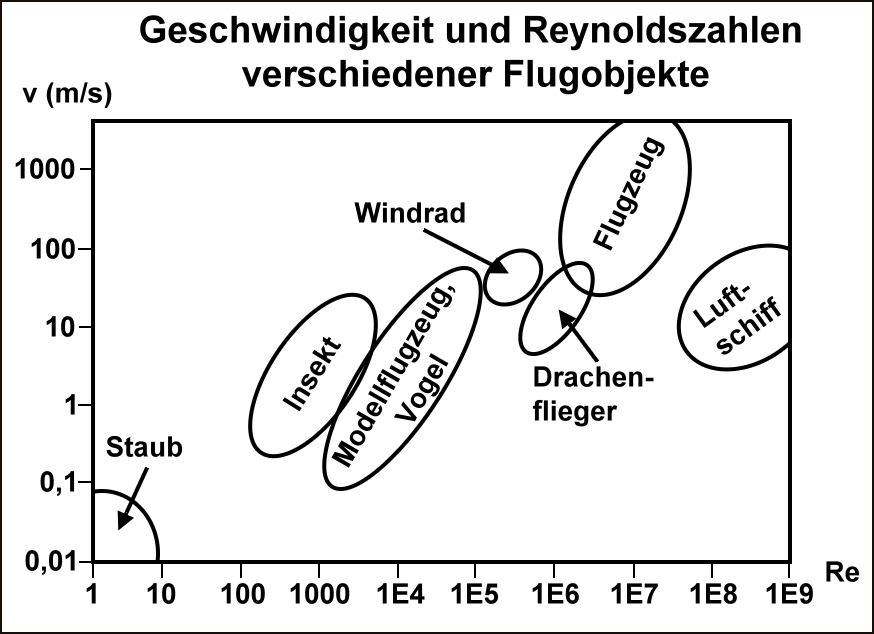
\includegraphics[width=0.80\textwidth]{Reynoldsflugrpd.png}
	\caption{Kurze Bildunterschrift}
	\label{fig:Reynoldsflugrpd}
\end{figure}
\begin{figure}[htbp]
	\centering
		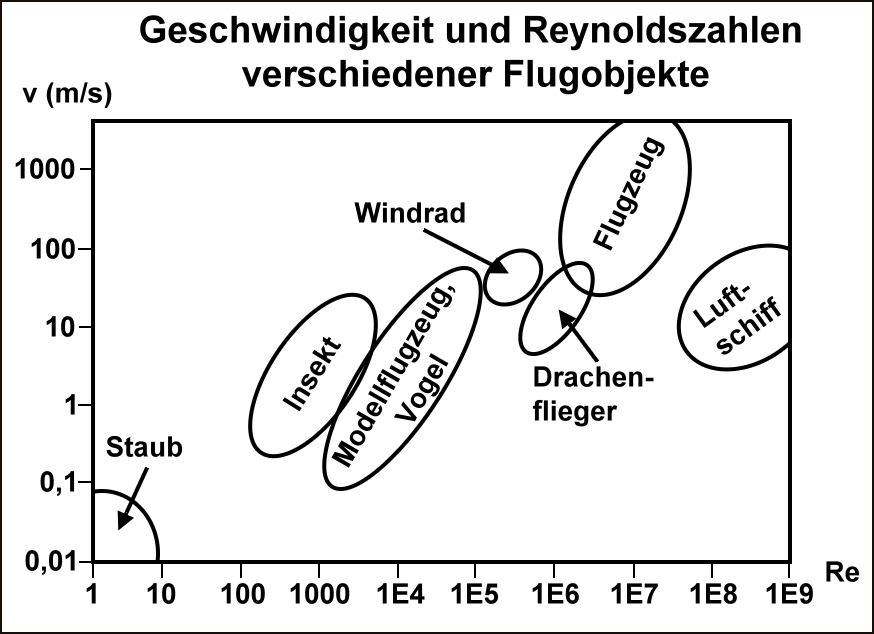
\includegraphics[width=0.80\textwidth]{Reynoldsflugrpd.png}
	\caption{Lange Bildunterschrift, welche die Länge einer Zeile überschreitet, bei mehrzeiligen Bildunterschriften wird der Zeilenabstand auf 1 reduziert.}
	\label{fig:Reynoldsflugrpd2}
\end{figure}

	\chapter{Beispiele}
\label{sec:Beispiele}
\section{Rohrströmung}
\label{sec:Rohrstroemung}
\subsection{Unterkapitel}
\label{sec:Unterkapitel}

Bei Rohrströmungen werden als charakteristische Größen üblicherweise der Innendurchmesser $L = d$, der Betrag der über den Querschnitt gemittelten Geschwindigkeit $u = u_m$ und die Viskosität des Fluids $\nu$ als Referenzgrößen verwendet, d.h.
\begin{equation}
	Re = \frac{u_m d}{\nu}  \ \ \ \ \ \ \ \mbox{.}
\end{equation}
Es gilt dann: $Re_k = 2300$.
Zu beachten ist, dass die kritische Reynoldszahl $Re_{k}$ nicht exakt den Übergang von einer laminaren zu einer turbulenten Strömung charakterisiert. Es ist in Experimenten gelungen, laminare Rohrströmungen mit $Re$ > 10000 zu erzeugen, ohne dass die Strömung turbulent geworden ist. Die kritische Reynoldszahl ist jedoch geeignet als Maß für den umgekehrten Übergang: Wenn die Strömung im Rohr verlangsamt wird, kann man bei $Re$ < 2300 von einer laminaren Strömung ausgehen. 
\subsubsection{Kritische Reynoldszahl}
\label{sec:KritischeReynoldszahl}
Die kritische Reynoldszahl $Re_k$, die den Übergang zwischen turbulenter und laminarer Strömung markiert, ist nicht nur abhängig von der Geometrie des Anwendungsfalles, sondern auch von der Wahl der charakteristischen Länge. Wird zum Beispiel der Rohrradius statt des Durchmessers der Strömung als charakteristisches Längenmaß einer Rohrströmung gewählt, halbiert sich der Zahlenwert $Re_k$, der dasselbe aussagen soll. Da die kritische Reynoldszahl ein Wert ist, der keinen blitzartigen Umschlag, sondern einen breiten Übergangsbereich der Strömungsverhältnisse markiert, ist der üblicherweise verwendete Zahlenwert nicht (2300/2) = 1150 sondern wird auf $Re_k \approx$ 1200 gerundet.

	\chapter{ Hinweise}
\label{sec:Hinweise}
\section{Allgemeine Hinweise}
\label{sec:AllgemeineHinweise}
Dies ist ein Beispiel für eine Aufzählung. Um den Abstand zwischen Aufzählung und Text sichtbar zu machen, verläuft dieser Text über zwei Zeilen
\begin{itemize}
	\item Strukturiertes Vorgehen bei der Problemlösung
	\item Kein Text zwischen Haupt- und Zwischenüberschrift
	\item Betrag und Einheit mit Leerzeichen, zum Beispiel 1 mm
	\item Zahlen bis Zehn und Einheiten ausschreiben
	\begin{itemize}
		\item im ersten Abschnitt oder im Abschnitt 1 nicht im 1. Abschnitt
		\item In einer Entfernung von einem Kilometer oder In einer Entfernung von L = 1 km, nicht In 1 km Entfernung 
		\item zehn Prozent Gewinn statt 10 \% Gewinn
		\end{itemize}
	\item Abkürzungen möglichst vermeiden, besser ausschreiben
	\begin{itemize}
	\item Zum Beispiel statt z.B.
\end{itemize}
\end{itemize}	
Dies ist der Text nach der Aufzählung. Auch hier kann man den Abstand zwischen Aufzählung und darauffolgenden Text sehen.
\clearpage
\section{Bilder untereinander und nebeneinander}
\label{sec:BilderUntereinander}
\subsection{Eine Bildunterschrift}
\label{sec:EineBildunterschrift}

\begin{figure}[ht]
  \centering
  \subfigure{
    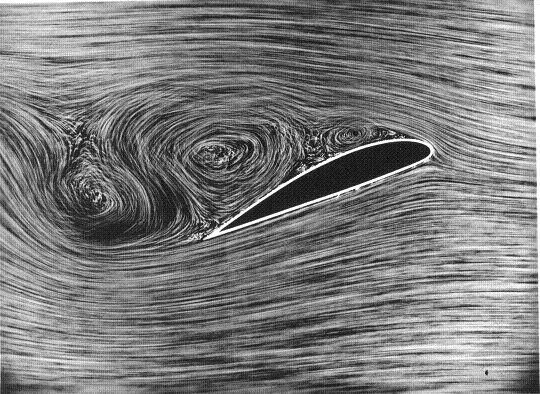
\includegraphics[width=0.5\textwidth]{stroemung1.PNG}  
  }
  \subfigure{
    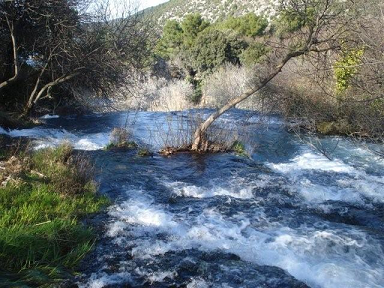
\includegraphics[width=0.35\textwidth]{stroemung2.PNG}  
  }
  \subfigure{
    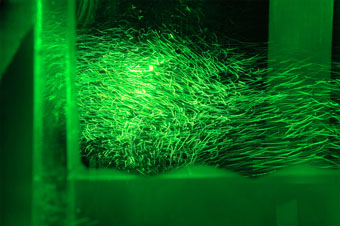
\includegraphics[width=0.25\textwidth]{stroemung3.PNG}  
  }
  \caption{Bildunterschrift}
  \label{fig:xyz1}
\end{figure} 
\clearpage

\begin{landscape}
\section{Querformat}
\label{sec:Querformat}
\begin{figure}[ht]
  \centering
  \subfigure{
    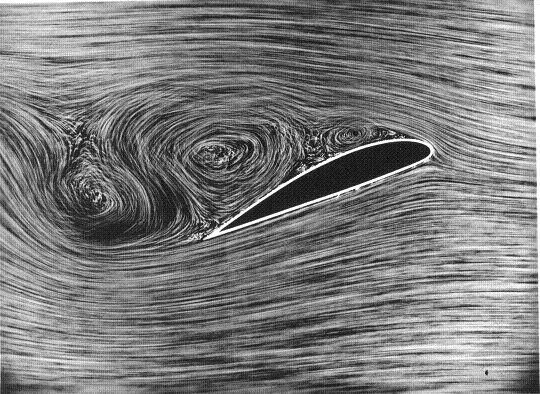
\includegraphics[width=0.3\textwidth]{stroemung1.PNG}
  }
  \subfigure{
    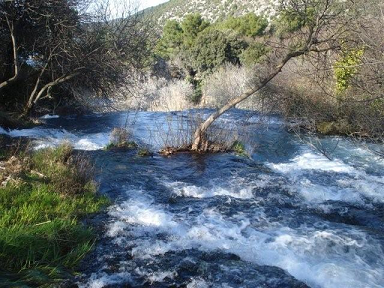
\includegraphics[width=0.3\textwidth]{stroemung2.PNG} 
  }
  \subfigure{
    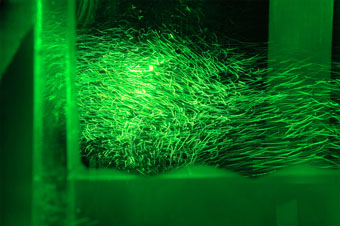
\includegraphics[width=0.3\textwidth]{stroemung3.PNG}
  }
  
  \caption{Bildunterschrift}
  \label{fig:xxxyyyzzzccc}
\end{figure}

\end{landscape}
	\chapter{Zusammenfassung und Ausblick}
\label{sec:ZusammenfassungUndAusblick}

Die Arbeit wird durch eine Zusammenfassung und einen Ausblick abgeschlossen. Dieser bildet in diesem Sinne das Gegenstück zur Einleitung. Ziel ist es, die dort beschriebenen Ziele und Wege kritisch zu beleuchten. \par
Hierbei ist es wichtig den Roten Faden im Auge zu behalten, d.h. einen problemlos nachvollziehbaren Weg durch das Dokument zu gehen, welcher bereits in der Einleitung übersichtshalber skizziert wurde.\par
Achten Sie am Ende auf die unterschriebene Selbstständigkeitserklärung sowie die Vollständigkeit des Dokuments.

  \clearpage
  \renewcommand{\bibname}{Literaturverzeichnis}
  \bibliographystyle{abbrv}
  \bibliography{literatur}

  \cleardoublepage
	\appendix
	\addchap{Anhang}
\label{ch:Anhang}
\refstepcounter{chapter}

Ein Beispiel für eine Herleitung oder Formel im Anhang.
\begin{equation}
	Re= \frac{\rho_l u_b d_e}{\eta_l} \ \ \ \ \ \ \ \mbox{.}
\end{equation}

Ein Beispiel für eine Tabelle im Anhang.
\begin{table}[htbp]
\caption{kurze Tabellenüberschrift}
	\label{tab:xyz3}
	\centering
	\footnotesize
	\sffamily
		\begin{tabular}{|c||c|c|}
			\hline
			Substanz & Rel. dyn. Viskosität & Rel. Dichte \\ \hline\hline
			 Wasser  &       $  1   $       & $    1   $  \\ \hline
			  Luft   &       $ 0,02 $       & $ 0,0013 $  \\ \hline
			  $x$    &       $  y   $       & $    z   $  \\ \hline
		\end{tabular}
\end{table}

Ein Beispiel für ein Bild im Anhang.
\begin{figure}[ht]
  \centering
    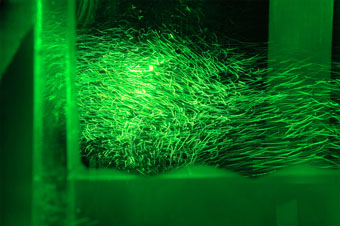
\includegraphics[width=0.47\textwidth]{stroemung3.PNG}
  \caption{Bildunterschrift}
  \label{fig:bild4}
\end{figure}

	\cleardoublepage
\chapter*{Selbstständigkeitserklärung}
\thispagestyle{empty}
Hiermit erkläre ich, dass ich die von mir am heutigen Tag der Professur für Strömungsmechanik eingereichte 
Diplomarbeit
%Interdisziplinäre Projektarbeit 
%(den) Großen Beleg (eingereichten)
zum Thema 
\begin{center}
\textit{Thema}
\end{center}
vollkommen selbstständig verfasst und keine anderen als die angegebenen Quellen und Hilfsmittel benutzt, sowie Zitate kenntlich gemacht habe.
\\[10mm]
Musterstadt, 00. Monat 20xx \\[1cm]
Max Mustermann


\end{document}
